\section{Contexto histórico e motivação}

%http://heroicrelics.org/info/v-2/v-2-cut-away.html
%https://v2rockethistory.com/?s=jet+vane

A tecnologia de controle de vetorização de empuxo (ou TVC, do inglês \textit{thrust vector control}) é chave para o setor aeroespacial, pois permite aproveitar o empuxo gerado pelo motor-foguete para aplicar um comando de atitude ao veículo. É uma tecnologia desenvolvida desde os primórdios da tecnologia de foguetes, com o míssil V2 sendo um marco notável no histórico do empuxo vetorial e dos foguetes. Este sistema, exibido na figura~\ref{fig:tvc_systems_jet_vanes}, utilizava lâminas de grafite (\textit{jet vanes}) inseridas na exaustão do motor principal para direcionar o escoamento de gases e produzir uma força lateral capaz de direcionar o míssil~\cite{V2jetvanes}.

\begin{figure}
    \centering
    \begin{subfigure}{.49\textwidth}
        \centering
        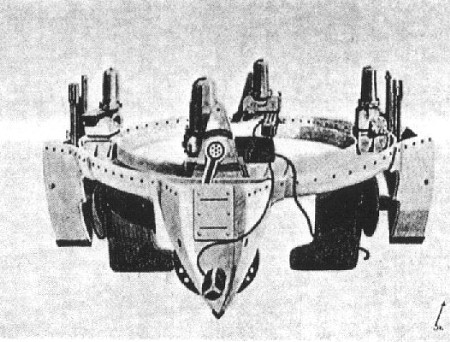
\includegraphics[width=.9\textwidth]{img/v2jetvanes.jpg}
        \caption{Sistema de \textit{jet vanes} do míssil V2~\cite{V2jetvanes}.}\label{fig:tvc_systems_jet_vanes}
    \end{subfigure}
    \hfill
    \begin{subfigure}{.49\textwidth}
        \centering
        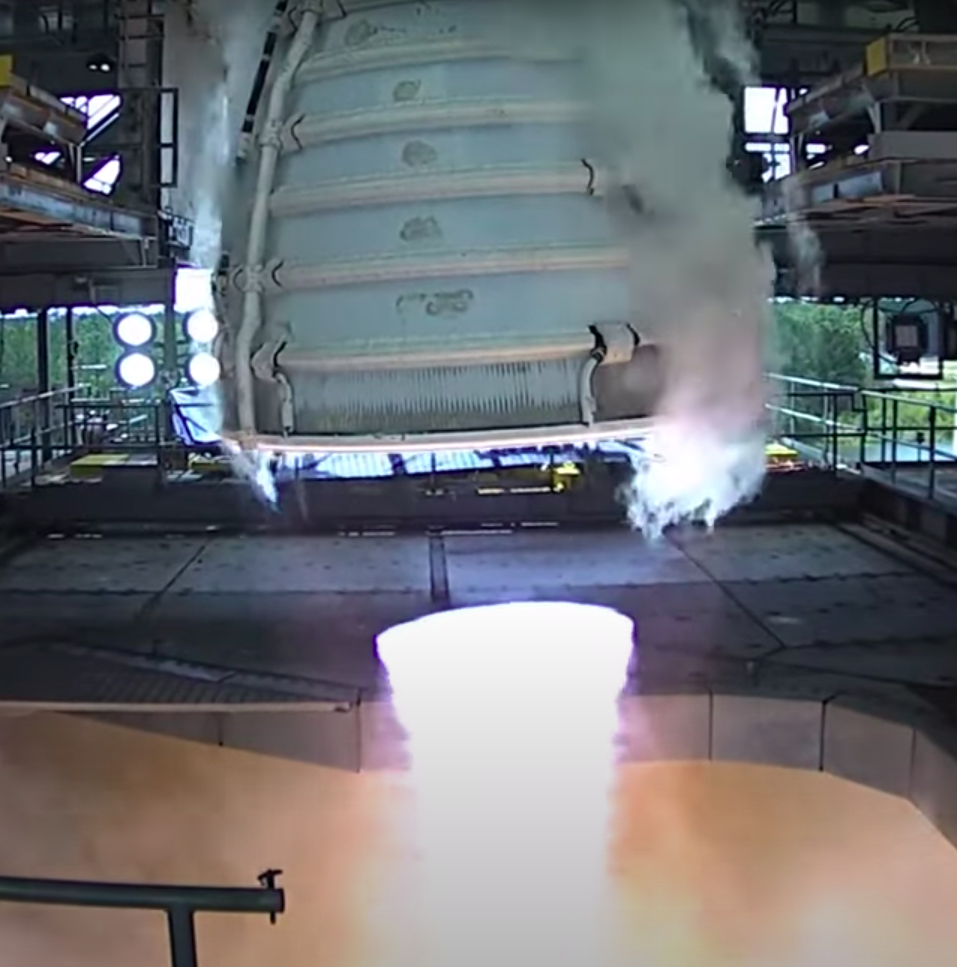
\includegraphics[width=.9\textwidth]{img/engine_gimbal.png}
        \caption{Sistema de \textit{gimbal} do motor RS-25 do foguete Artemis~\cite{RS25Gimbal}.}\label{fig:tvc_systems_gimbal}
    \end{subfigure}
    \caption{Exemplos de sistemas com empuxo vetorial.}
\end{figure}

Outros sistemas de vetorização de empuxo foram desenvolvidos após a Segunda Guerra Mundial, tanto para aplicações militares como para lançadores de satélites, cada uma com seus \textit{trade-offs} de engenharia. Uma alternativa de alto desempenho e alta complexidade mecânica muito comum atualmente é a articulação esférica, ou \textit{gimbal}, da tubeira do motor. Um sistema \textit{gimbal}, do motor RS-25 desenvolvido para o ônibus espacial e reaproveitado para o programa Artemis, é exibido em ação na figura~\ref{fig:tvc_systems_gimbal}.

Os sistemas de vetorização de empuxo são fundamentais para a estabilidade e para o seguimento de trajetória dos foguetes. Defeitos de manufatura podem introduzir desalinhamentos angulares e lineares de empuxo, que devem ser compensados pelo sistema de controle de empuxo vetorial. Também são fundamentais para o controle dos veículos em baixas velocidades, regime no qual aletas fornecem pouca ou nenhuma autoridade sobre o veículo, permitindo que se elimine a necessidade de trilhos de lançamento. Naturalmente, também funcionam no vácuo espacial. Este trabalho busca, portanto, iniciar uma linha de pesquisa brasileira sobre o assunto.

\section{Introdução Teórica}\label{sec:intro}
A propulsão de motores-foguete é baseada na força de reação gerada pela aceleração de uma massa em um sentido oposto ao sentido desejado da força propulsiva. Tecnologicamente, este conceito é implementado com o uso de escoamentos de fluidos compressíveis, acelerados por diferenças de pressão presentes no sistema. Do ponto de vista da engenharia aeroespacial, faz-se necessário conhecer algumas métricas de eficiência que possam ser aplicadas em um projeto. Assim, a propulsão é uma área derivada da mecânica, termodinâmica e engenharia.

No vácuo, a força propulsiva, ou empuxo, é uma função do fluxo mássico do sistema e da velocidade de ejeção de propelente (derivada diretamente da segunda lei de Newton). Para sistemas propulsivos em uma atmosfera, deve ser adicionado um termo corretivo referente à diferença de pressão entre a atmosfera e o escoamento ejetado. Assim, o empuxo pode ser dado, em primeira aproximação, por~\cite{Sutton}:
\begin{equation}
    \label{eq:thrust_basic}
    F = \dot{m} v_e + (p_e - p_{\mathrm{amb}}) A_e
\end{equation}
onde \(F\) é a força propulsiva, \(\dot{m}\) é o fluxo mássico de propelente, \(v_e\) é a velocidade de exaustão do propelente, relativa ao veículo, \(p_e\) é a pressão local na saída da tubeira, \(A_e\) é a área de saída da tubeira e \(p_{\mathrm{amb}}\) é a pressão ambiente. Observa-se que a equação~\ref{eq:thrust_basic} assume valores médios para a seção da saída tubeira.

A razão de expansão é um parâmetro geométrico de um sistema propulsivo, dado por
\begin{equation}
    \label{eq:exp_ratio}
    \varepsilon = \frac{A_e}{A_t}
\end{equation}
onde \(A_e\) é a área da saída da tubeira e \(A_t\) é a área da seção transversal da garganta. Após a garganta, o escoamento está supersônico, e deverá ser acelerado por um aumento da área da seção transversal da tubeira~\cite{anderson}. Assim, a razão de expansão influencia diretamente a velocidade de saída do propelente, descrevendo quanta energia interna (pressão e temperatura) do propelente foi convertida em energia cinética. Razões de expansão maiores implicam em maiores velocidades de saída \(v_e\). No entanto, para motores que operam em uma atmosfera, deve-se atentar também para o fato de que \(p_e\) depende da razão de expansão. Se a razão de expansão for grande demais, haverá uma grande perda de empuxo devido ao segundo termo da equação~\ref{eq:thrust_basic} e, em casos mais graves, descolamento do fluxo e vibrações estruturais intensas. Assim, busca-se otimizar a razão de expansão para uma condição específica de pressão ambiente.

Um parâmetro de desempenho usado para comparar a eficiência mássica do sistema propulsivo é o impulso específico. Ele mede o impulso imprimido ao veículo por peso de propelente ou, analogamente (supondo regime estacionário), a força gerada por vazão de peso de propelente~\cite{Sutton}:
\begin{equation}
    \label{eq:Isp}
    I_{\text{sp}} = \frac{\int^T_0 F dt}{g_0 \int^T_0 \dot{m}dt} = \frac{F}{g_0 \dot{m}}
\end{equation}
onde \(g_0=9,80665\;\mathrm{m}\,\mathrm{s}^{-2}\)~\cite{CGPM}. Este fator \(g_0\), a gravidade padrão, foi introduzido para permitir que a unidade do impulso específico seja \(s\), permitindo a fácil comunicação de valores de impulso específico entre instituições que usam o sistema métrico e o sistema imperial. Assim, sistemas propulsivos muito energéticos e eficientes terão, de modo geral, impulso específico alto, pois conseguem imprimir altas velocidades à massa de reação. Inversamente, sistemas pouco energéticos, como os de gás frio, terão impulsos específicos baixos.

Outro parâmetro útil é o coeficiente de empuxo \(C_F\). Ele mede a amplificação de empuxo advinda da expansão do escoamento supersônico na tubeira do foguete. Ou seja, ele mede a razão entre o empuxo real do sistema e a força que seria obtida aplicando-se a pressão de câmara na área da garganta~\cite{Sutton}:
\begin{equation}
    \label{eq:C_F}
    C_F = \frac{F}{p_c A_t}
\end{equation}

Se o coeficiente de empuxo mede a eficiência da tubeira, a velocidade característica \(C^*\) mede a eficiência do conjunto câmara e propelente. A velocidade característica é dada por~\cite{Sutton}:
\begin{equation}
    \label{eq:cstar}
    C^* = \frac{p_c A_t}{\dot{m}}
\end{equation}

A partir das equações~\ref{eq:C_F} e~\ref{eq:cstar} é possível deduzir uma relação muito útil para projeto, que permite o cálculo fácil da vazão mássica necessária:
\begin{equation}
    \label{eq:mdot}
    \dot{m} = \frac{F}{C^* C_F}
\end{equation}

As relações dadas anteriormente assumem que o escoamento está estagnado na câmara de empuxo. Na prática, buscam-se razões \(\frac{A_c}{A_t} \gg 1\) para satisfazer esta hipótese. A literatura recomenda valores mínimos de 4 ou 6~\cite{Sutton}.

%https://software.nasa.gov/software/LEW-17687-1
%https://rocketcea.readthedocs.io/en/latest/
A termodinâmica é capaz de fornecer expressões analíticas para todas as grandezas apresentadas aqui, supondo-se gás perfeito, ausência de reação química e escoamento quasi-unidimensional. No entanto, para uma análise química e termodinâmica mais precisa, busca-se o software CEA NASA~\cite{ceanasa}, que calcula dos parâmetros propulsivos a partir de certas condições de operação e entradas termodinâmicas do propelente. Com este software, é possível calcular os valores de \(C_F\) e \(C^*\) para um sistema propulsivo com hipóteses menos rígidas que as exigidas pela teoria de escoamento quasi-unidimensional. Este software foi usado a partir de uma interface programática~\cite{rocketcea}.

O sistema de \textit{jet vanes} escolhido para este trabalho consiste na imersão de uma lâmina em escoamento supersônico, de modo que formar-se-ão ondas de choque próximas ao bordo de ataque da lâmina. Para escoamentos tridimensionais não uniformes e assimétricos, ou seja, o caso de uma lâmina defletora imersa na exaustão de uma tubeira de foguete, analisar as ondas de choque e expansão formadas torna-se extremamente complicado. No entanto, é possível apresentar alguns resultados obtidos da literatura para casos mais simples, mas ainda relevantes. 

Primeiramente, observa-se que a natureza das ondas de choque é bastante dependente da geometria do bordo de ataque do corpo em questão. A figura~\ref{fig:shock_waves}~\cite{vandyke} mostra um caso de choque colado em uma cunha fina e um caso de choque descolado em uma esfera (corpo rombudo). Para corpos de espessura finita, estas ondas sempre vão existir, mas serão tão mais fortes quanto mais rombudo o corpo for. As ondas de choque são responsáveis pelo \textit{arrasto de onda}, uma forma de arrasto não-viscoso que se apresenta em escoamentos supersônicos. No caso de lâminas defletoras, esse arrasto atuará no sentido de diminuir a força propulsiva gerada pelo sistema como um todo.

\begin{figure}[htbp]
    \centering
    \begin{subfigure}{0.49\textwidth}
        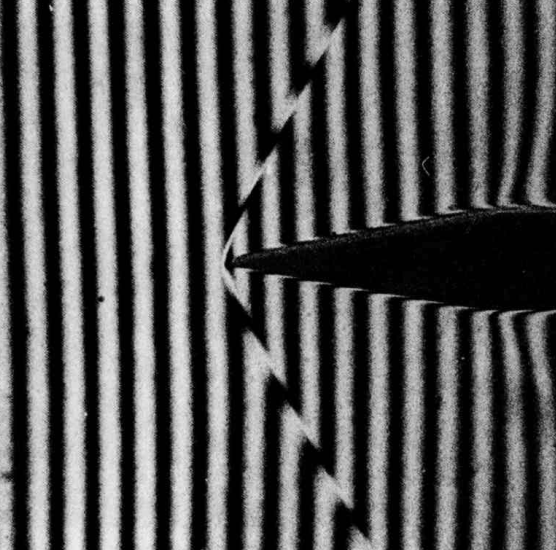
\includegraphics[width=\textwidth]{img/attached_shock.png}
    \end{subfigure}
    \begin{subfigure}{0.49\textwidth}
        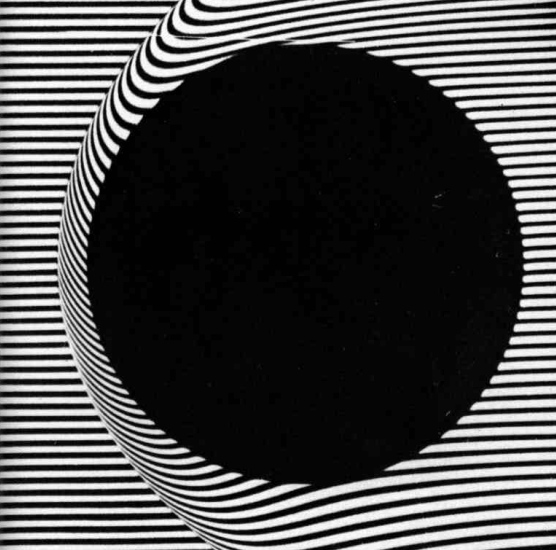
\includegraphics[width=\textwidth]{img/dettached_shock.png}
    \end{subfigure}
    \caption{Tipos diferentes de ondas de choque que podem se estabelecer no bordo de ataque de um corpo imerso em escoamento supersônico: colado e descolado.}\label{fig:shock_waves}
\end{figure}

Para placas infinitamente planas em ângulos pequenos, imersas em escoamentos supersônicos uniformes e estacionários, situação ilustrada na figura~\ref{fig:supersonic_flat_plate}, é possível encontrar equações analíticas para a sustentação \(L\) (força perpendicular ao escoamento) e para o arrasto \(D\) (paralela ao escoamento), em função da área da superfície \(S\), do ângulo de ataque \(\alpha \) e da densidade, velocidade e número de Mach do escoamento não perturbado (\(\rho_\infty \), \(V_\infty \) e \(M_\infty \))~\cite{anderson}:
\begin{align}
    L &= \frac{1}{2} \rho_\infty V_\infty^2 S \frac{4\alpha}{\sqrt{M_\infty^2-1}} \label{eq:sslift} \\
    D &= \frac{1}{2} \rho_\infty V_\infty^2 S \frac{4\alpha^2}{\sqrt{M_\infty^2-1}}
\end{align}

\begin{figure}[htbp]
    \centering
    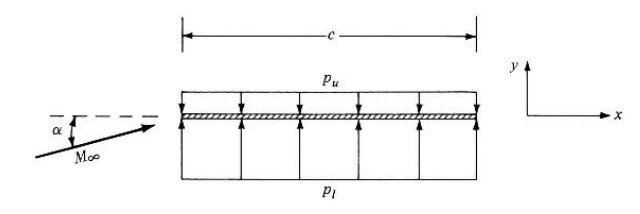
\includegraphics[width=\textwidth]{img/supersonic_flat_plate.png}
    \caption{Diagrama de placa plana em escoamento supersônico em pequenos ângulos}\label{fig:supersonic_flat_plate}
\end{figure}

Dessa forma, na prática espera-se que a força lateral (análoga à sustentação) gerada pela lâmina defletora seja proporcional à sua deflexão, e que o arrasto da lâmina seja não nulo para deflexão nula (devido à espessura não nula) e que este aumente quadraticamente com a deflexão.

Para aplicações de controle, é comum modelar a dinâmica do sistema como um modelo de espaço de estados linear invariante no tempo~\cite{fbsys}:
\begin{align}
    \dot{\textbf{x}} &= A\textbf{x} + B\textbf{u} \\
    \textbf{y} &= C\textbf{x} + D\textbf{u}
\end{align}
onde \(\textbf{x}\) é o vetor de estado do sistema, \(u\) é o vetor de entradas e \(\textbf{y}\) é o vetor de saídas. \(A\), \(B\), \(C\) e \(D\) são, respectivamente, as matrizes de dinâmica, controle, sensor e direta. A vetorização de empuxo é uma opção de sistema de controle para veículos aeroespaciais, de modo que ela constitui uma forma de entrada para o sistema. Sendo assim, é necessário caracterizar o vetor \(\textbf{u}\) e a matriz \(B\) referentes ao sistema de controle.

A vetorização de empuxo inclui no vetor de entradas de um sistema a posição de lâmina defletora \(\delta \). Sua influência sobre o sistema, sob hipótese de linearidade, justificada pela equação~\ref{eq:sslift}, depende, dentre outros fatores específicos da aplicação, das \textit{derivadas de controle} de força lateral e momento:
\begin{align}
    F_{x\delta} &= \frac{\mathrm{d}F_x}{\delta} \\
    M_{\delta} &= \frac{\mathrm{d}M}{\delta}
\end{align}

\section{Objetivos}

Este trabalho buscou caracterizar as derivadas de controle de um sistema de vetorização de empuxo. Como objetivos intermediários, foram estabelecidos o desenvolvimento de um motor foguete a gás frio de pequena escala (\(2\)--\(5\,\mathrm{N}\)), o desenvolvimento de um sistema de vetorização de empuxo baseado em lâmina defletora (\textit{jet vane}), a caracterização empírica das forças geradas pelo sistema, bem como a identificação de parâmetros de projeto e \textit{trade-offs} de engenharia relacionado à vetorização de empuxo.